\chapter{Experiments and Results}
\label{cha:experiments}

\section{Experimental Plan and Setup}
\label{sec:experimental-plan-and-setup}

\begin{comment}
Trying and failing is a major part of research. However, to have a chance of success you need a plan driving the experimental research, just as you need a plan for your literature search. Further, plans are made to be revised, and this revision ensures that any further decisions made are in line with the work already completed.

The plan should include what experiments or series of experiments are planned and what questions the individual or set of experiments aim to answer. Such questions should be connected to your research questions, so that in the evaluation of your results you can discuss the results wrt to the research questions.
\end{comment}

The experiments conducted for this report have been planned to answer the research questions described in \autoref{sec:goals-and-research-questions}.

\subsection[RQ1: Determining the Potential of LLM-based GIS analysis]{\rqref{rq:llm-potential}: Determining the Potential of LLM-based GIS analysis}

\rqref{rq:llm-potential} differs from \rqref{rq:overlay-analysis} and \rqref{rq:external-tools} in that it is more open-ended. The tests will try to display what abilities \acrshort{acr:gpt}-4 has geospatial tasks out of the box, without providing it with any context or external tools.

\subsubsection{Ability to Perform Geospatial Analysis}

Tests were performed to assess ChatGPT's ability to perform geospatial analysis. The testing approach is inspired by the work of \cite{robertsGPT4GEOHowLanguage2023} (see \autoref{subsec:gis-with-llms}), who did experiments with increasing difficult on \acrshort{acr:gpt}-4 to characterize what \acrshort{acr:gpt}-4 knows about the geographical world, highlighting both capabilities and limitations. These focused on \acrshort{acr:gpt}-4's general geospatial awareness, and were not concerned with \acrshort{acr:gis}-related tasks. Therefore, I will refer to \cite{robertsGPT4GEOHowLanguage2023} when highlighting its somewhat surprising geospatial awareness abilities, and focus my efforts to displaying its potential for use in the world of \acrshort{acr:gis}. I will do this by constructing various tests that try to reflect its GIS knowledge.

I will use the Elveg 2.0 dataset \citep{thenorwegianmappingauthorityElveg2019}, along with cadastral data. In order to assess ChatGPT's ability to read and understand different data formats, the data will be provided in both \acrshort{acr:sosi}, \acrshort{acr:gml}, and GeoJSON format. Datasets for the first two formats were downloaded from \url{https://geonorge.no}, while the GeoJSON datasets were created using a custom Bash script which converts from \acrshort{acr:gml} to GeoJSON using the \texttt{ogr2ogr} program from \acrshort{acr:gdal}. The Elveg 2.0 dataset contains a range of different layers for different types of geometries. In order to simplify the experiments, only the layer named "Fartsgrense" (eng. "Speed limit") was used fro Elveg 2.0.

Below are the questions that were asked, in rising order of predicted complexity.

\begin{enumerate}
    \item \enquote{Provide a summary of the file contents, highlighting the file's most salient features.}
    \item \enquote{Provide a visual representation of the file contents.}
    \item \enquote{Find the mean location of the building locations.}
    \item \enquote{Extract all roads with a speed limit greater than or equal to 80 km/h.}
    \item \enquote{Select all buildings located within 50 metes of a high-speed road (speed limit >= 80 km/h).}
    \item \enquote{Find the area best suited for expansion to accommodate residential buildings.}
          % \item \enquote{Assess the environmental impact of the proposed expansion.}
\end{enumerate}
\label{enum:gpt-gis-questions}

Some follow-up questions are added when needed, in order help the model understand the questions or when it stops and asks for permission to go forth with analysis.

\subsubsection{Data Access}

Another important thing to test is the issue of providing ChatGPT with relevant files on which it can perform analysis. ChatGPT Plus users will have access a range of advanced features, including web browsing with Bing, Dall-E Image Generation, and Code Interpreter. The latter of these allows the user to manually upload files into the chat instance and perform advanced analyses on the contents of these, which is what was used to upload the datasets for the tests above. While this is very powerful, having to manually upload files poses some limitations. A more flexible system should be capable of accessing web \acrshortpl{acr:api} in real time.

A dataset containing the border of Drammen Municipality was used to test compare ChatGPT's ability to perform analyses on manually uploaded data, versus data handed through it from passing a URL address. The data conforms to the GeoJSON standard and contains a FeatureCollection object with a single Feature, namely the border. When file/URL has been provided, ChatGPT is simply asked to present a visual presentation of its contents.

\subsection[RQ2: Testing ChatGPT's Ability to Perform Overlay Analysis using OGC API Features]{\rqref{rq:overlay-analysis}: Testing ChatGPT's Ability to Perform Overlay Analysis using \acrshort{acr:ogc} \acrshort{acr:api} Features}

Experiments on \rqref{rq:overlay-analysis} will require three different elements:

\begin{enumerate}
    \item Provide ChatGPT with \acrshort{acr:api} URL(s) to relevant data collections corresponding with the \acrshort{acr:ogc} \acrshort{acr:api} - Features specification
    \item Prompts to ChatGPT-4 using the "Code Interpreter" beta feature
    \item Gold standard/expected output for the given combination of input data and prompts
\end{enumerate}

These experiments will be limited to the collections found at \url{https://alenos-tester001.azurewebsites.net/}. This example \acrshort{acr:ogc} \acrshort{acr:api} was created by Norkart's Alexander Salveson Nossum for with the purpose of testing \acrshort{acr:ogc} \acrshort{acr:api} Features on Norwegian data. It was created using \texttt{pygeoapi}\footnote{\url{https://pygeoapi.io/}}, which is a Python server implementation of the \acrshort{acr:ogc} \acrshort{acr:api} suite of standards. It allows for deployment of a RESTful \acrshort{acr:ogc} \acrshort{acr:api} endpoint using OpenAPI, GeoJSON, and HTML.

\subsection[RQ3: Testing ChatGPT's Ability to To Use External Tools]{\rqref{rq:external-tools}: Testing ChatGPT's Ability to Use External Tools}

Experiments on \rqref{rq:external-tools} will test different tools and techniques intended to give an \acrshort{acr:llm} access to up-to-date information and external tools (see \autoref{subsec:retrieval-automented-generation} on \acrlong{acr:rag}). The main focus will be on how one can use a tool like \hyperref[subsubsec:langchain]{LangChain} hook up a conversational \acrshort{acr:ai} with sophisticated functionality found in various \acrshort{acr:gis} software.

\section{Experimental Results}
\label{sec:experimentalResults}

\subsection[Results for RQ1 Tests]{Results for RQ1 Tests \rqref{rq:llm-potential}}

\subsection{Ability to Perform Geospatial Analysis}

Preliminary experiments showed that ChatGPT's Code Interpreter is unable to read and write \acrshort{acr:sosi} files. It was unable to manipulate the data directly and was also unable to convert the file a more suitable format, failing to convert it GeoJSON using \acrshort{acr:gdal}'s \texttt{ogr2ogr}. \acrshort{acr:sosi} is therefore excluded from \autoref{tbl:data-format-tests}, which shows the successfulness of ChatGPT to perform analyses on various file formats.

\begin{table}
    \centering
    \begin{tabular}{l|p{0.2\textwidth}p{0.2\textwidth}p{0.2\textwidth}}
        \toprule
                               & \textbf{GML} & \textbf{GeoJSON} & \textbf{Shapefile} \\
        \midrule
        Summary                & Yes          & Partially        & Partially          \\
        Plotting               & When guided  & When guided      & Yes                \\
        Mean location          & When guided  & Yes              & No                 \\
        Filtering              & No           & Yes              & Yes                \\
        Buffer + Intersect     & No           & No               & No                 \\
        Planning for expansion & No           & Partially        & No                 \\
        \bottomrule
    \end{tabular}
    \caption{The first three rows of the training dataset}
    \label{tbl:data-format-tests}
\end{table}

The Code Interpreter did not manage to properly analyze the \acrshort{acr:gml} data without guidance. It created a parser that was difficult to use for further analysis. When guided into using the GeoPandas library, which accepts \acrshort{acr:gml} data, it managed to plot the contents and calculate a centroid. The buffering and intersection task \enquote{was interrupted due to its time-consuming nature}, and it did not make an attempt at solving the planning task due to inability to analyze the \acrshort{acr:gml} files.

As for the GeoJSON data, ChatGPT had difficulties reading the files and could not provide a good summary consistently. It \textit{was} able to plot the data, but that had to be done in separate responses for each of the datasets. It was able to find the high-speed roads, but could not figure out which buildings were within a 50-meter buffer of these. However, when asked to plan for expansion to accommodate residential buildings, it managed to achieve a result close to what was expected in the "Buffer + Intersect" task. It accomplished this by creating a grid and figuring out which grid cells were within 50 meters of a high-speed road. This did not extract a subset of the building points---which would have been the desired output---but it had some minor value in terms of visualization (see \autoref{fig:planning-plot-from-geojson}). Though the result is useful, it was closer than in the \acrshort{acr:gml} attempt to what would be an expected response.

Using the shapefile formatted data, ChatGPT was able to produce a decent summary of the data, but the attribute names were cut off after about 10 characters. It was, however, able to produce quite good visual representations of both dataset, colouring the roads differently by their speed limits and the buildings by their building type.

\begin{figure}
    \centering
    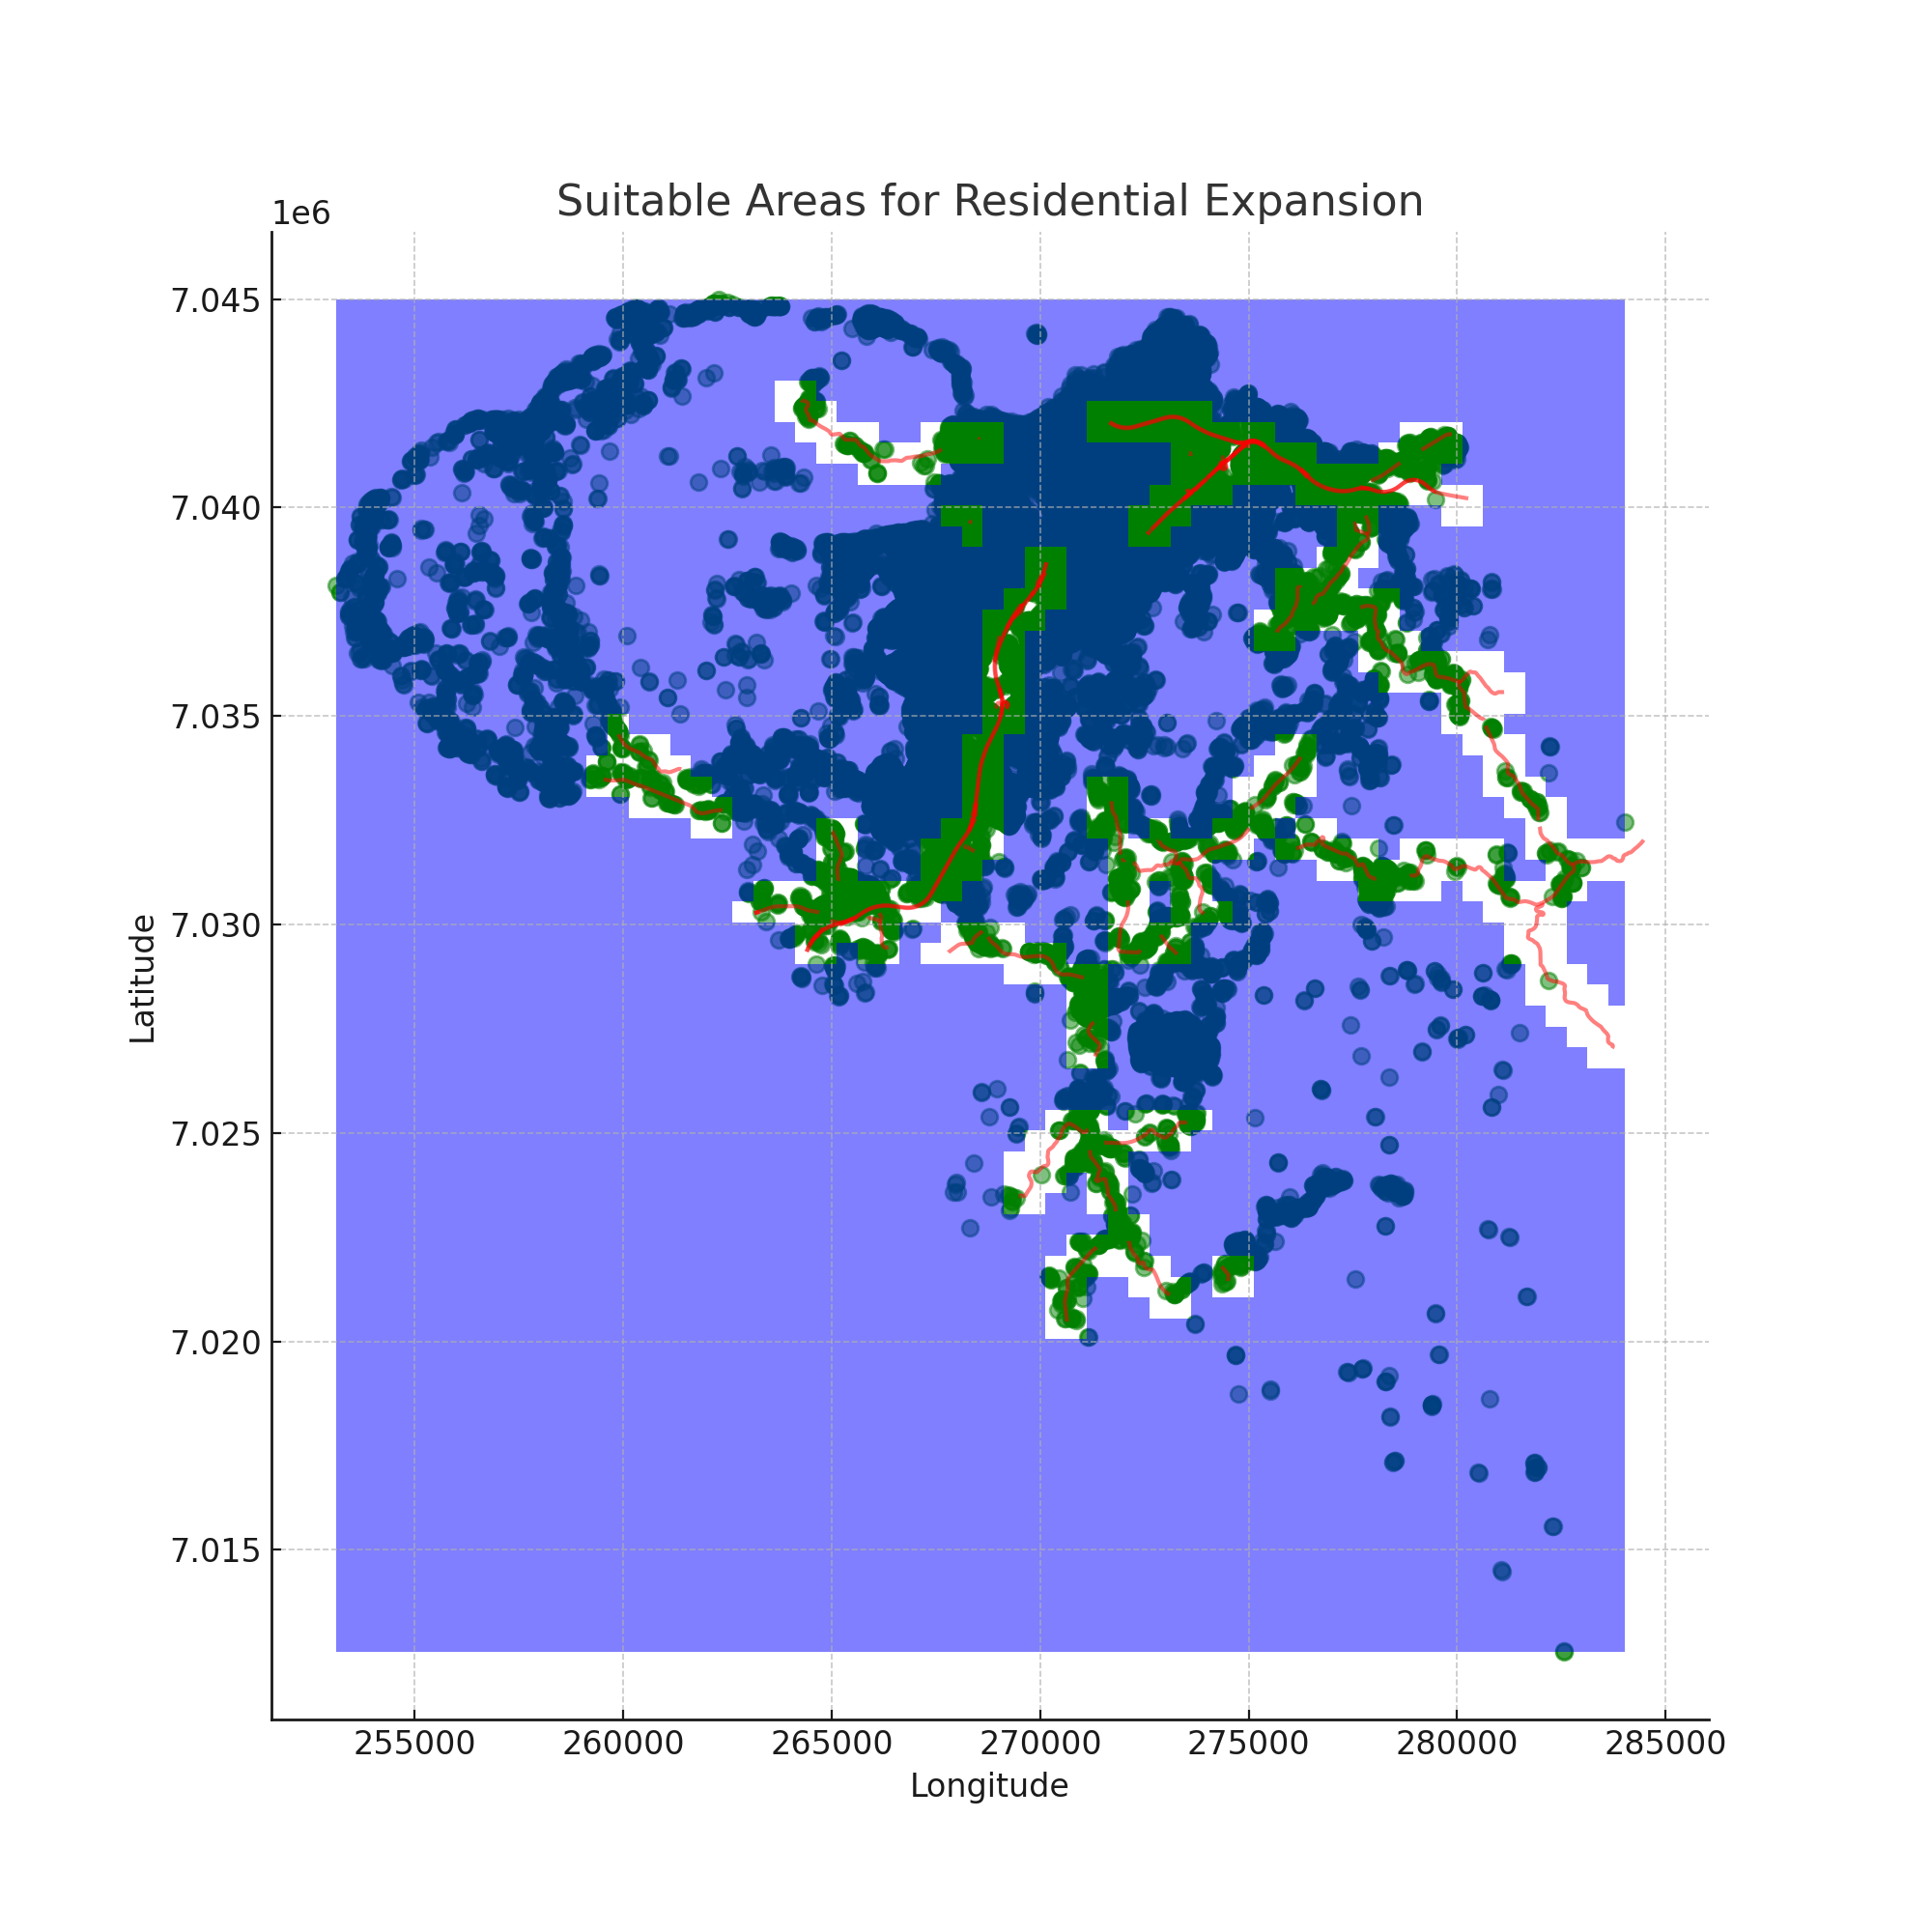
\includegraphics[width=\textwidth]{../figs/residential_expansion_areas_map.png}
    \caption{The result of ChatGPT when asked to \enquote{Find the area best suited for expansion to accommodate residential buildings}, using provided GeoJSON datasets. Potentially suitable areas for residential expansion  are depicted in blue.}
    \label{fig:planning-plot-from-geojson}
\end{figure}

\subsection{Data Access}


\subsection[Results for RQ1 Tests]{Results for RQ1 Tests \rqref{rq:llm-potential}}
\subsection[Results for RQ1 Tests]{Results for RQ1 Tests \rqref{rq:llm-potential}}







\begin{comment}
Results should be clearly displayed and should provide a suitable representation of your results for the points you wish to make.
Graphs should be labelled in a legible font. If more than one result is displayed in the same graph, then these should be clearly marked.
Please choose carefully rather than presenting every result. Too much information is hard to read and often hides the key information you wish to present. Make use of statistical methods when presenting results, where possible to strengthen the results.
Further, the format of the presentation of results should be chosen based on what issues in the results you wish to highlight.
You may wish to present a subset in the experimental section and provide additional results in an appendix.
Point out specifics here but save the overall/general discussion to the Discussion chapter.
\end{comment}

\glsresetall
